\documentclass[a4paper, 12pt]{scrartcl}

\usepackage[utf8]{inputenc}
\usepackage[ngerman]{babel}
\usepackage[T1]{fontenc}
\usepackage{amsmath}
\usepackage{braket}
\usepackage{amssymb}
\usepackage{graphicx}
\usepackage{wrapfig}


\author{Sebastian Steinhäuser}

\begin{document}

\begin{center}
\Large{\textbf{Spezialisierungsbericht}}
\\
\vspace{1cm}
\Huge{\textbf{Computersimulation aktiver Random-Walks auf perkolierendem Cluster}}
\\
\vspace{1cm}
\Large{Sebastian Steinhäuser}

\includegraphics[width=0.8\textwidth]{DLR.png}
\end{center}
\begin{center}
Betreut durch Thomas Voigtmann und Julian Reichert
\end{center}
\newpage
\tableofcontents
\newpage
\section{Perkolation}
\subsection{Was ist Perkolation?}
In diesem Bericht geht es stets um Perkolation auf einem Quadratgitter in zwei Raumdimensionen. In diesem Fall gibt es zwei geläufige Perkolationsmodelle, Knotenperkolation (engl. 'site-percolation') und Kantenperkolation (engl. 'bond-percolation'), hier wird immer über Knotenperkolation gesprochen. In folgender Abbildung \footnote{https://de.wikipedia.org/wiki/Perkolationstheorie, 21.10.2019} wird der Unterschied zwischen Knoten- und Kantenperkolation bildlich dargestellt.
\begin{figure}[h!]
\centering
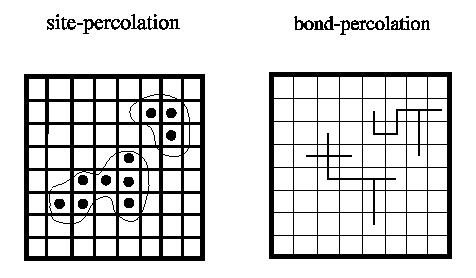
\includegraphics[scale=0.6]{Percolation1.jpg}
\caption{Knoten- und Kantenperkolation}
\end{figure}
\vspace{0,5cm}
\\
Das Quadratgitter wird zufällig mit einer Wahrscheinlichkeit $1-p$ geblockt (Es ist Konvention die Wahrscheinlichkeit das ein Platz frei ist mit $p$ zu bezeichnen, diese Konvention möchte ich hier erhalten.), geblockte Plätze können nicht besetzt werden. Man kann sich geblockte Plätze wie Wände eines Labyrinths vorstellen, durch die der Random-Walker später nicht hindurch kommt.  
\\
Nun definiert man einen Cluster als eine Gruppe benachbarter Quadrate die begehbar sind, also nicht geblockt. Man nennt einen Cluster perkolierend, wenn sich der Cluster von einer Kante zur gegenüberliegenden Kante erstreckt, ähnlich wie Wasser durch eine Kaffeemaschine (engl. 'percolator') perkoliert/sickert. Vereinfacht gesagt kann der Random-Walker sich unendlich ausbreiten und ist nicht 'eingesperrt'. Man kann sich nun leicht Vorstellen, dass wenn kaum Felder geblockt sind (also $p$ nahe $1$) sich auf dem (unendlich großen) Quadratgitter stets ein perkolierender Cluster finden lässt und wenn kaum Felder begehbar sind (also $p$ nahe $0$) sich nie ein perkolierender Cluster finden lässt. Es gibt dazwischen eine sogenannten kritischen Wert $p=p_c \approx 0.5928$ \footnote{D. Stauffer, Perkolationstheorie, Seite 5} bis zu welchem das unendliche Quadratgitter perkoliert, auch Perkolationsschwelle oder englisch percolation-threshold genannt.
\noindent Historisch geht die Perkolationstheorie (engl. 'percolation theory') auf Paul Flory und Walter H. Stockmayer zurück, die sie während des Zweiten Weltkriegs entwickelten, um Polymerisationsprozesse zu beschreiben. Der Polymerisationsprozess kommt durch das Aneinanderreihen von Molekülen zustande, die dadurch Makromoleküle bilden. Der Verbund solcher Makromoleküle führt zu einem Netzwerk von Verbindungen, die sich durch das ganze System ziehen können.\footnote{Zitiert aus: https://de.wikipedia.org/wiki/Perkolationstheorie, 21.10.2019}
\\
\noindent Üblicherweise wird der Beginn der Perkolationstheorie mit einer Publikation von Broadbent  und Hammersley aus dem Jahre 1957 in Verbindung gebracht, in welcher der Name eingeführt wurde, und in welcher sie mit den oben erläuterten geometrischen und wahrscheinlichkeitstheoretischen Konzepten mathematischer behandelt wurde. Hammersley erwähnt in seiner persönlichen Geschichte der Perkolation in 'Percolation Structures and Processes', dass die (damals) neuen Computer, die für die Wissenschaftler dieser Zeit zugänglich wurden, einer der Gründe für die Entwicklung der Perkolationstheorie waren: Hier handelte es sich um Probleme, bei denen die Computer nützlich werden konnten.\footnote{Zitiert aus: D. Stauffer, Perkolationstheorie, Seite 3-4}

\subsection{Perkolation auf dem Computer}
Es ist selbstverständlich nicht möglich ein unendlich großes Quadratgitter mit zufällig geblockten und freien Gitterplätzen auf dem Computer zu erzeugen, daher wird hier stets ein endliches Quadratgitter(auf dem Computer in Form einer Matrix/Array gespeichert) und mit periodischen Randbedingungen ausgestattet. Um perkolierende Cluster dieser zufällig erzeugten Matrix zu finden nutzt man den sogenannten Hoshen-Kopelmann-Algorithmus.\footnote{https://www.ocf.berkeley.edu/~fricke/projects/hoshenkopelman/hoshenkopelman.html, 21.10.2019}
Dieser Algorithmus lässt sich am besten an einem Beipiel erklären. Im nachfolgenden Bild sind freie Felder grau und geblockte Felder weiß, graue Felder die an einer Kante verbunden sind (wo der Random-Walker also von einem Feld ins andere kann) werden mit dem selben Label versehen.
\begin{figure}[h!]
\centering
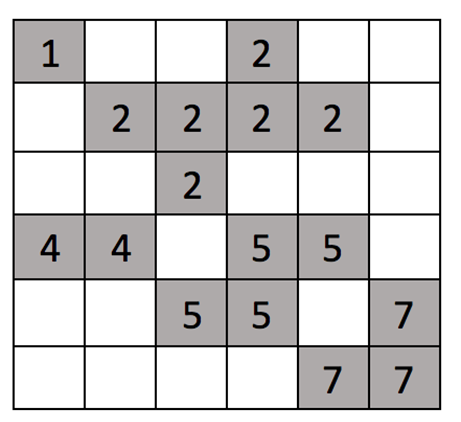
\includegraphics[scale=0.5]{H-K_algorithm.png}
\caption{Veranschaulichung des Hoshen-Kopelmann-Algorithmus}
\end{figure}
\vspace{0,5cm}
\newpage
\noindent Geht ein Cluster von einem Rand zum gegenüberliegenden Rand, also tritt an diesen beiden Kanten das selbe Label auf so perkoliert dieser Cluster in der endlichen Matrix (ohne periodische Randbedingungen!). Dies bedeuted aber nicht das der Cluster im Sinne der peridischen Randbedingungen perkoliert. 
\\
Hier ist noch Arbeit zu tun!

\section{Random-Walk in ungeordneten Medien}

\subsection{"Normeler"\ Random-Walk}
Der Random-Walk auf dem freien Quadratgitter unterliegt bekanntlich normaler Diffusion, das heißt, dass das mittlere quadratische Verschiebung (engl. mean squared displacement), welches im weiteren mit $msd$ abgekürzt wird, linear mit der Anzahl an Schritten anwächst. Im kontinuierlichen Fall gilt die bekannte Formel:
\begin{align*}
msd(t)\equiv \langle \delta r^2 (t) \rangle =2dDt\ ,
\end{align*}
wobei $d$ die Dimension und $D$ der Diffusionskoeffizient sind.

\subsection{Random-Walk auf dem Perkolationsgitter}
Das Perkolationsgitter bei dem nur ein zufälliger Bruchteil der Gitterplätze begehbar sind und die anderen geblockt sind ist ein besonders einfaches Modell für ein ungeordnetes Medium. Eine spannende Frage - die in den 70er und 80er Jahren des vergangenen Jahrhunderts durch eine Vielzahl von Computersimulationen geklärt wurde - ist, wie sich ein Random-Walker auf so einem unregelmäßigen Perkolationgitter für verschiedene $p$ ($=$ Wahrscheinlichkeit das ein Gitterplatz begehbar ist) verhält, speziell geht man von einem Potenzgesetz:
\begin{align*}
msd(t) \sim t^{2 \nu},\ \ \nu=1/d_w
\end{align*} 
aus, wobei $\nu$ als Diffusionsexponent bezeichnet wird und $d_w$ als 'fraktale Dimension'. Der im Feld der weichen Materie bekannte französische Physiker Pierre-Gilles de Gennes nannte diese Fragestellung 1976 die 'Ameise im Labyrinth'.\footnote{D. Stauffer, Perkolationstheorie, Kapitel 1.4} 
\\ 
\noindent Zuerst überlegt man sich leicht die beiden Extremfälle $p$ nahe $1$ und $p$ nahe $0$. Im ersten Fall ($p \approx 1$) erwartet man sofort, dass $\nu$ nahe $1/2$ ist, da es kaum 'Hindernisse' gibt und der Random-Walk nahezu ungestört laufen kann. Anders herum, bei $p$ nahe $0$ erwartet man, dass es keine perkolierenden Cluster gibt, somit ist der Random-Walker 'eingesperrt' in sogenannte 'Taschen', damit das $msd$ beschränkt und somit $\nu \rightarrow 0$ für lange Zeiten. Besonders spannend ist dieses Problem also in der Nähe der Perkolationsschwelle $p=p_c$, hier findet sich ein Diffusionskoeffizient, der weder $1/2$ noch $0$ ist. Gefen, Aharony und Alexander nannten diesen Effekt, dass der Diffusionskoeffizient weder normal  ($\nu = 1/2$) ist noch verschwindet, 'anormale Diffusion'.\footnotemark[6] Diese anormale Diffusion wird auf für Zwischenwerte wie zum Beispiel $p=0.7$ gefunden, der Random-Walker spürt auch eine leichte fraktale Struktur und hat daher einen Exponenten zwischen $1/2$ und dem auf dem Perkolationsgitter $\nu_{pc}$.

\subsection{'all-cluster-' und 'percolating-cluster average'}

Es gibt im Allgemeinen zwei Varianten wie man $\nu_{pc}$ auffassen kann, man mittelt über zufällige Startpunkte auf dem zufällig geblockten Quadratgitter oder man mittelt über Startwerte die nur auf dem perkolierenden Cluster liegen ('all-cluster average' und 'percolating-cluster average'). Es ist zu erwarten, dass der Exponent bei dem 'all-cluster average' unter dem Exponenten des 'percolating-cluster average' liegt, da beim 'all-cluster average' auch in sogenannten Taschen gestartet wird in denen das $msd$ beschränkt ist. Die aktuell bekannten 'Literaturwerte' sind $d_w^{a.c.} \approx 3.036$ und $d_w^{p.c.} \approx 2.878$, woraus sich $\nu_{pc}^{a.c.} \approx 0.329$ und $\nu_{pc}^{p.c.} \approx 0.347$ ergeben.\footnote{P. Grassberger, Phys. A 262, 251 (1999)} In dieser Spezialisierung wurde versucht diese Werte durch Monte-Carlo-Simulation (MC) zu reproduzieren, es wurde eine Gitterlänge $L=1000$ verwendet und die Perkolationsschwelle als $p_c = 0.592\ 746$ angenommen. Es wurden zu beiden Mittelungsvarianten über $100$ Läufe auf je $100$ zufälligen Matrizen gemittelt. Die Läufe waren je $10^6$ MC-Schritte lang und wurden auf einem ($10$er-) logarithmischen Grid gespeichert mit 48 Speicherstellen. 
\begin{figure}[h!]
\centering
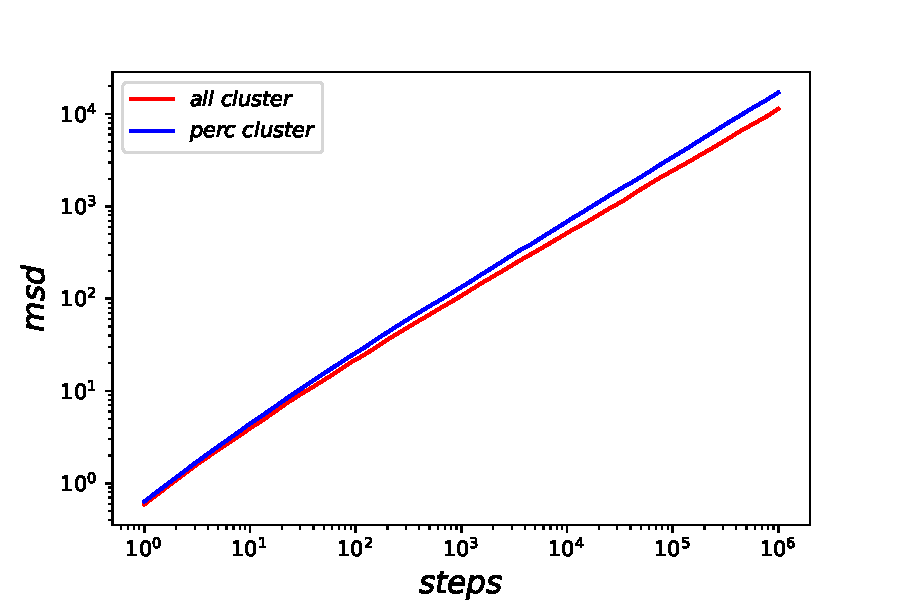
\includegraphics[scale=0.9]{acpc_fig.pdf}
\caption{Ergebnisse meiner python3 MC-Simulation, der 'all-cluster average' ist in rot, der 'percolating-cluster average' in blau}
\end{figure}
\vspace{0,5cm}
\newpage
\noindent Die Exponenten wurden über einen $scipy.optimize.curve\_fit$ als $\nu_{pc}^{a.c.}$ und $\nu_{pc}^{a.c.}$ bestimmt. Die Methode den Exponenten durch einen fit zu bestimmen hat sich als deutlich stabiler herausgestellt als das bestimmen der Ableitung durch eine 'central-difference' oder gar 'forward-difference' Methode, welche unter sehr hohen numerischen Fehler leiden, da zwei sehr große Zahlen von einander abgezogen werden deren Differenz klein ist. Dieses Problem ist bekannt als 'catastrophic cancellation'. Nimmt man Werte die weiter auseinander liegen (also ein größeres $h$) so wird die Ableitung ebenfalls sehr ungenau, da der Fehler quadratisch ('central-difference') beziehungsweise linear ('forward-difference') in Abstand $h$ wächst. Die logarithmische Ableitung stellt eine weitere zufridenstellende Alternative da, da das erste Problem der kleinen Differenz großer Zahlen umgangen wird. 

\subsection{Self-Avoiding Walk auf dem Perkolationsgitter}
Self-Avoiding Walks (kurz: SAW), also Random-Walks die niemals zu einem zuvor besuchten Gitterplatz zurückkehren sind ein Standardthema in der Physik der weichen Materie, da sie ein Modell für Polymerketten geben. Der Exponent $\nu^{SAW}$ des $msd$ beim SAW ist daher von besonderem Interesse, da er eine Verbingung zwischen mittlerer Größe eines Polymers und der Anzahl der Kettenglieder schafft:
\begin{align*}
\tilde R \equiv \sqrt{\langle R^2 \rangle} \sim N^{\nu^{SAW}},
\end{align*} 
wobei $\tilde R$ der Durchmesser des Polymers ist.
\\
Nun lässt sich auch leicht die Frage formulieren wie sich ein SAW auf dem Perkolationsgitter ausbreitet. Der normale Random-Walk ist langsamer geworden, genauer: $\nu_{pc} \equiv \nu_{pc}^{p.c.} < 1/2$, im Gegensatz dazu wird der SAW auf dem Perkolationsgitter schneller. In anderen Computersimulationen wurde $\nu^{pcSAW} \approx 0.78$ gefunden wohingegen $\nu^{SAW}=3/4=0.75$ ist. Der SAW ist ein wichtiger Vergleich zu dem 'aktiven' Random-Walk.


\end{document}